
\documentclass{ppgeesa}

%%%%%%%%%%%%%%%%%%%%%%%%%%%%%%%%%%%%%%%%%%%%%%%%%%%%%%%%%%%%%%%%%%%%%%%%%%%%%%%%%%%%%%%%%%%%%%%%%%%%%%%%%%%%%%%%%

\usepackage[latin1]{inputenc}
\usepackage{graphicx}
\usepackage{hyperref}
\usepackage{tikz}
\usepackage{amsmath}
\usepackage{listings}
\makeatletter
\def\@xobeysp{ }
\makeatother

\lstset{ %
language=Matlab,                % choose the language of the code
basicstyle=\footnotesize,       % the size of the fonts that are used for the code
numbers=none,                   % where to put the line-numbers
numberstyle=\footnotesize,      % the size of the fonts that are used for the line-numbers
stepnumber=2,                   % the step between two line-numbers. If it's 1 each line 
                                % will be numbered
numbersep=5pt,                  % how far the line-numbers are from the code
backgroundcolor=\color{white},  % choose the background color. You must add \usepackage{color}
showspaces=false,               % show spaces adding particular underscores
showstringspaces=false,         % underline spaces within strings
showtabs=false,                 % show tabs within strings adding particular underscores
frame=false,	                % adds a frame around the code
tabsize=2,		                % sets default tabsize to 2 spaces
captionpos=b,                   % sets the caption-position to bottom
breaklines=true,                % sets automatic line breaking
breakatwhitespace=true,         % sets if automatic breaks should only happen at whitespace
title=\lstname,                 % show the filename of files included with \lstinputlisting;
                                % also try caption instead of title
escapeinside={\%*}{*)}         % if you want to add a comment within your code
%morekeywords={*,...}            % if you want to add more keywords to the set
}
\lstset{caption=Descriptive Caption Text,label=DescriptiveLabel}

% reference : http://en.wikibooks.org/wiki/LaTeX/Hyperlinks
\hypersetup{
    bookmarks=true,												% show bookmarks bar?
    unicode=false,												% non-Latin characters in Acrobat�s bookmarks
    pdftoolbar=true,											% show Acrobat�s toolbar?
    pdfmenubar=true,											% show Acrobat�s menu?
    pdffitwindow=false,											% window fit to page when opened
    pdfstartview={FitH},										% fits the width of the page to the window
    pdftitle={Modelagem e identifica��o de sistemas},			% title
    pdfauthor={Tassiano Neuhaus (tassianors@gmail.com)},		% author
    pdfsubject={M�todos param�tricos de identifica��o de sistemas},   % subject of the document
    pdfcreator={Tassiano Neuhaus},								% creator of the document
    pdfproducer={Producer},										% producer of the document
    pdfkeywords={Identifica��o de sistemas} {M�todos param�tricos}, % list of keywords
    pdfnewwindow=true,											% links in new window
    colorlinks=true,											% false: boxed links; true: colored links
    linkcolor=black,											% color of internal links
    citecolor=red,												% color of links to bibliography
    filecolor=magenta,											% color of file links
    urlcolor=blue												% color of external links
}

%%%%%%%%%%%%%%%%%%%%%%%%%%%%%%%%%%%%%%%%%%%%%%%%%%%%%%%%%%%%%%%%%%%%%%%%%%%%%%%%%%%%%%%%%%%%%%%%%%%%%%%%%%%%%%%%%


\begin{document}

\title{Modelagem e Identifica��o de sistemas lineares}

\author{Tassiano Neuhaus\\
{\small Universidade Federal do Rio Grande do Sul - Departamento de Engenharia El�trica\\Av. Osvaldo Aranha, 103 - Bairro Bom Fim CEP: 90035-190 - Porto Alegre - RS - Brasil}\\
}%\thanks{Tassiano Neuhaus, tassianors@gmail.com, tel +55-51-91760154}

\maketitle

\thispagestyle{empty}\pagestyle{empty}

\begin{abstract}
%===============================================================================
% ABSTRACT
%===============================================================================

Neste trabalho ser� apresentado diversos meios para a identifica��o de sistemas
lineares. Existem dois grupos principais de m�todos para esta identifica��o, sendo
um deles conhecido como {\it{identifica��o n�o param�trica}} onde existem infinitos
par�metros para serem estimados e que normalmente � utilizado para identifica��o de
fun��es gr�ficas. Outro m�todo � conhecido como {\it{identifica��o param�trica}} onde
o n�mero de par�metros a ser estimado � finito. Este �ltimo m�todo ser� mais abordado
neste trabalho, por possuir uma aplicabilidade maior devido a possibilidade de estimar 
processos em fun��es matem�ticas que descrevem o comportamento do sistema muitas vezes
com mais informa��o que os m�todos gr�ficos.

Para este trabalho ser� utilizado um processo de controle de posi��o angular, controlado
por um motor de corrente continua. Ser�o apresentados diversos m�todos de identifica��o 
e ao fim ser� feito um comparativo entre os resultados obtidos.


\end{abstract}

\begin{IEEEkeywords}
Identifica��o de sistemas lineares, m�todos param�tricos.
\end{IEEEkeywords}

%===============================================================================
\section{Introdu��o}

Neste trabalho ser� apresentado um sistema de para controle de posi��o angular,
manipulado por um motor de corrente continua (DC). O objetivo principal, � estimar
os valores das vari�veis existentes no modelo escolhido para representar este sistema.

Inicialmente ser� explicado o processo de escolha do modelo que representa a din�mica
deste sistema (Se��o (\ref{sec:modelling})). Ser� explicitado quais considera��es sobre
o sistema foram feitas para se obter o modelo que ser� utilizado nas se��es seguintes, 
para determinar os par�metros.

Em seguida, ser� utilizado o m�todo dos M�nimos quadrados (MQ), para estimar o sistema, 
considerando-se para isso que o ruido sobre o sistema sofre influ�ncia dos mesmos polos
que est�o na planta, ou seja, que o modelo para o sistema se comporta como um modelo ARX.
Nesta mesma se��o (\ref{sec:mmq}) ser� apresentado os resultados para o mesmo sistema, 
baseado nos mesmos dados, mas para um modelo que n�o representa o sistema f�sico, ou que 
n�o consegue representa-lo.

Na se��o (\ref{sec:iv}) ser� apresentado o m�todo das vari�veis instrumentais, para estimar
os valores do par�metro para o modelo. Da mesma forma que para o m�todo dos MQ, ser�
utilizado um modelo que n�o representa o sistema real, e este m�todo ser� aplicado para 
determinar a qualidade dos resultados obtidos.

Ao fim, ser� apresentado uma breve discuss�o sobre os resultados obtidos em ambos os m�todos
utilizados, e as considera��es finais.


\section{Modelagem do sistema}
\label{sec:modelling}
%===============================================================================

O objetivo da modelagem de um sistema � encontrar um modelo (fun��o com par�metros
livres) que consiga representar o sistema f�sico de forma completa. A partir do
conhecimento do sistema f�sico, fazem-se considera��es sobre o sistema, para simplifica-lo
a fim de tornar o modelo matem�tico o mais simples poss�vel, mas que ainda represente
o sistema real, com a margem de preciosidade definida, pela quantidade e qualidade 
das simplifica��es aplicadas para chegar-se ao modelo matem�tico do sistema.
\cite{system_identification}

\subsection{Sistema F�sico}
%===============================================================================

O sistema f�sico em estudo neste trabalho, � um sistema para controle de posi��o, onde 
o atuador � um motor de corrente continua (DC). Desta forma a entrada do sistema 
� a tens�o aplicada sobre os terminais do motor em Volts [V], e a sa�da � a posi��o
angular do motor em radianos [rad].

Na Figura (\ref{fig:motor_system}) pode ser vista a representa��o el�trica e mec�nica
do motor em quest�o.

\begin{figure}[htbp]
	\center
	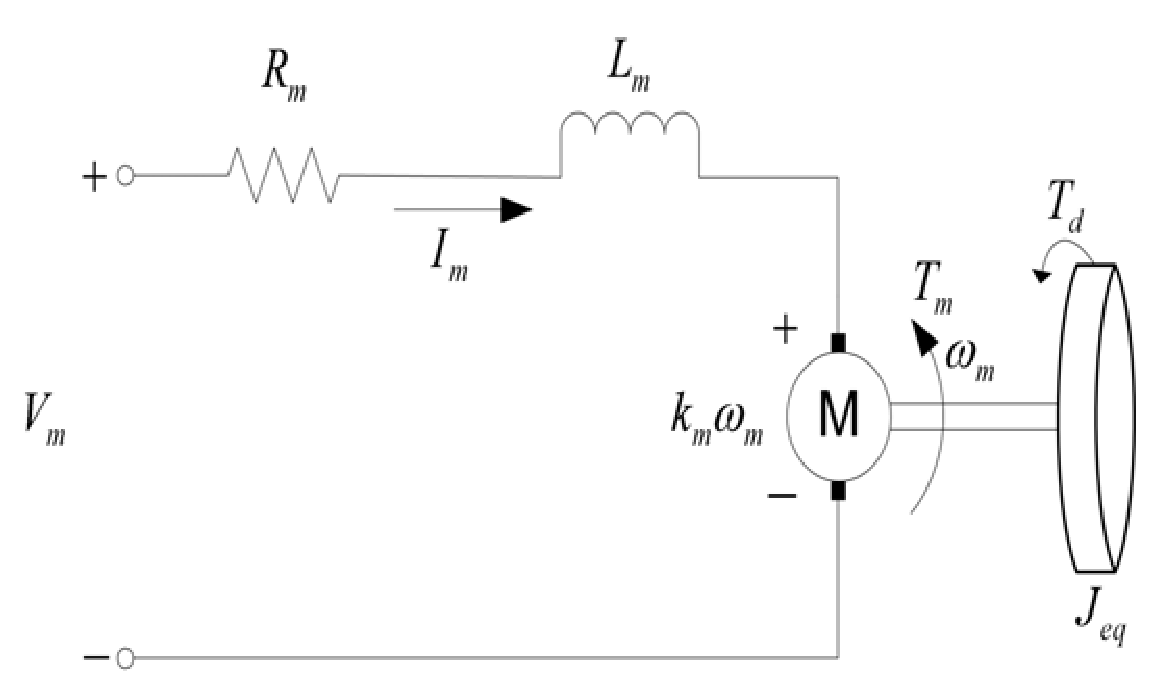
\includegraphics[width=0.7\columnwidth]{figures/motor_system.eps}
	\caption{Representa��o el�trica e mec�nica do motor}
	\label{fig:motor_system}
\end{figure}

As vari�veis consideradas para a modelagem s�o as apresentadas abaixo:

\begin{itemize}
	\item $\omega$ = Velocidade do motor.
	\item \it{v} = Tens�o aplicada na armadura.
	\item \it{ia} = corrente de armadura.
	\item \it{L} = Indut�ncia da armadura.
	\item \it{e} = Forca contra eletromotriz = $K_{2} \omega$
	\item \it{R} = Resist�ncia do enrolamento da armadura.
	\item \it{T} = Torque aplicado = $K_{i} ia$
	\item \it{J} = Momento de inercia da carga.
	\item \it{f} = Atrito viscoso no eixo.
\end{itemize}

Tem-se desta forma as duas equa��es que descrevem o sistema para a parte el�trica
(\ref{eq:motor_elet}) e mec�nica (\ref{eq:motor_mec}).

\begin{equation}
V-R\cdot Ia - L\frac{\mathrm{d} Ia}{\mathrm{d} x}-e = 0
\label{eq:motor_elet}
\end{equation}

\begin{equation}
J \dot{\omega}= T-f\omega
\label{eq:motor_mec}
\end{equation}

A partir destas equa��es diferenciais pode-se chegar ao sistema de equa��es de estado 
descrito em (\ref{eq:motor_eq_estados}).

\begin{equation}
\begin{matrix}
\begin{bmatrix}
\dot{Ia}\\ 
\dot{\omega} \\
\dot{\theta}
\end{bmatrix}= &
\begin{bmatrix}
-R/L & -K_2/L & 0\\ 
K_i/J & -f/J & 0 \\
0 & 1 & 0
\end{bmatrix}&
\begin{bmatrix}
Ia\\ 
\omega \\
\theta
\end{bmatrix} + &
\begin{bmatrix}
1\\ 
0\\
0
\end{bmatrix} V
\end{matrix}
\label{eq:motor_eq_estados}
\end{equation}

Com este sistema de equa��es de estado, � poss�vel obter-se as fum�es de transfer�ncias,
que descrevem o sistema, para uma entrada e uma sa�da. Na equa��o (\ref{eq:motor_pos_tf}) 
apresenta-se a fun��o de transfer�ncia do motor, que relaciona a posi��o com a tens�o de entrada
do motor.

\begin{equation}
G(s)=\frac{k_1/JL}{s(s+f/L)(s+R/L)+s\;k_1 k_2/JL}
\label{eq:motor_pos_tf}
\end{equation}

Devido a din�mica do sistema mec�nico ser muito menor que a din�mica do sistema el�trico, 
pode-se desconsiderar a influencia do polo el�trico do sistema, ficando a fun��o de transfer�ncia
como a seguir:

\begin{equation}
G(s)=\frac{\frac{k_1}{JL}}{s(s+\frac{fL+k_1 k_2}{JL})}
\nonumber
\end{equation}

A equa��o anterior (\ref{eq:motor_pos_tf}) representa o comportamento da posi��o angular do motor
baseado na entrada de tens�o aplicada sobre seus terminais. Esta Fun��o de transfer�ncia descreve este
comportamento em tempo continuo, nosso sistema � digital e com isso precisamos de uma
representa��o discreta para esta mesma fun��o, para isso pode ser utilizados diversos m�todos, como
Euler backward, Euler forward, entre outras aproxima��es. Iremos neste trabalho utilizar a aproxima��o
de Euler Forward (\ref{eq:modelling_forward}).

\begin{equation}
s\cong \frac{(z-1)}{T_S}
\label{eq:modelling_forward}
\end{equation}

Desta forma, chega-se a uma fun��o de transfer�ncia (\ref{eq:motor_pos_tf_disc}).

\begin{equation}
G(z)=\frac{a}{(z-1)(z-b)}
\label{eq:motor_pos_tf_disc}
\end{equation}

Onde :

\begin{equation}
\begin{matrix}
a=\alpha \;T_S^2\\ \;\\
b=\beta T_S-1\\ \;\\
\alpha = \frac{k_1}{JL}\\ \;\\
\beta = \frac{fL+k_1 k_2}{JL}
\end{matrix}
\nonumber
\end{equation}

Com $T_S$ sendo a frequ�ncia de amostragem utilizada.

Desta forma chega-se a uma modelagem do sistema que relaciona a posi��o em fun��o da tens�o aplicada
sobre o motor. Para tanto foi considerado que a din�mica da parte mec�nica do sistema � muito mais
predominante que a din�mica da parte el�trica, podendo esta ser desconsiderada para que o sistema 
se torne um pouco mais simples.


\section{Modelagem n�o param�trica}
\label{sec:non_parametric}
%===============================================================================




\section{Modelos param�tricos simples}
\label{sec:parametric}
%===============================================================================



\section{M�todo dos m�nimos quadrados}
\label{sec:mmq}
%===============================================================================

O m�todo dos m�nimos quadrados (MMQ) � um dos mais conhecidos e mais utilizados 
nas mais diversas �reas da ci�ncia e tecnologia. A origem da ideia b�sica pode ser
encontrada nos trabalhos de Gaus sobre o estudo astron�micos. \cite{aguirre}

\subsection{Sistema com solu��o �nica}
%===============================================================================

Considerando-se que o sistema que ser� observado seja linear e invariante no tempo.
Se a fun��o $f$ que descreve o sistema for n�o linear o sistema poder� em principio 
ser identificado por modelos n�o lineares. Com base nestas restri��es temos que:

\begin{equation}
\begin{matrix}
\begin{matrix}
\begin{bmatrix}
y_1\\ 
y_2\\ 
\vdots \\ 
y_n
\end{bmatrix} = &
\begin{bmatrix}
x_1 & x_2 & \cdots  & x_n
\end{bmatrix} &
\begin{bmatrix}
\theta_1\\ 
\theta_2\\ 
\vdots \\ 
\theta_n
\end{bmatrix}
\end{matrix}
\\ \\
y=X\theta
\end{matrix}
\nonumber
\end{equation}

Com $X \in \Re^{nxn}$. Desde que $X$ seja n�o singular � poss�vel determinar $\theta$:

\begin{equation}
\theta=X^{-1}y
\label{eq:mmq_base}
\end{equation}

\subsection{Sistema sobredeterminado}
%===============================================================================

Para sistemas sobredeterminados onde $ N > n$, A vari�vel $X$ da equa��o (\ref{eq:mmq_base}) fica
$X \in \Re^{Nxn}$. Como esta matriz n�o � quadrada, n�o � poss�vel de ser invertida. Multiplicando-se
a equa��o (\ref{eq:mmq_base}) por $X^T$ tem-se: \cite{aguirre}

\begin{equation}
X^Ty=X^TX\theta
\nonumber
\end{equation}

De onde vem:

\begin{equation}
\theta = [X^T X]^{-1} X^T y
\label{eq:mmq}
\end{equation}

O m�todo dos m�nimos quadrados minimiza o crit�rio apresentado em (\ref{eq:mmq_j}).

\begin{equation}
J(\theta)=\frac{1}{2N}\sum_{t=1}^{N}[y(t)-\hat{y}(t, \theta)]^2
\label{eq:mmq_j}
\end{equation}

Onde $\hat{y}(t, \theta)$ � a predi��o do sistema e pode ser representado como abaixo:

\begin{equation}
\hat{y}(t, \theta)=\theta^T \phi(t)
\nonumber
\end{equation}

Desta forma pode se dizer que o sistema real � o pr�prio sistema estimado mais algum 
erro de estimativa:

\begin{equation}
y(t) = \hat{y}(t, \theta) +e(t)=\theta^T \phi(t) + e(t)
\nonumber
\end{equation}

\subsection{Estruturas de modelagem}
%===============================================================================

De forma gen�rica modelos para descri��o de sistemas podem ser representados como em 
(\ref{eq:mmq_generic_model}).

\begin{equation}
A(q, \theta)Y(t)=\frac{B(q, \theta)}{F(q, \theta)}U(t)+\frac{C(q, \theta)}{D(q, \theta)}e(t)
\label{eq:mmq_generic_model}
\end{equation}

Onde:

\begin{equation}
\begin{matrix}
A(q, \theta)=1+a_1 q^{-1}+a_2 q^{-2}+\cdots +a_{na} q^{-na}\\
B(q, \theta)=b_1 q^{-1}+b_2 q^{-2}+\cdots +b_{nb} q^{-nb}\\ 
C(q, \theta)=1+c_1 q^{-1}+c_2 q^{-2}+\cdots +c_{nc} q^{-nc}\\ 
D(q, \theta)=1+d_1 q^{-1}+d_2 q^{-2}+\cdots +d_{na} q^{-nd}\\ 
F(q, \theta)=1+f_1 q^{-1}+f_2 q^{-2}+\cdots +f_{nf} q^{-nf} 
\end{matrix}
\nonumber
\end{equation}

Baseado nestas informa��es existem modelos onde apenas alguns destes polin�mios s�o 
diferentes de 1. Na Tabela (\ref{tab:model}) s�o apresentados alguns destes modelos
mais comumente utilizados.

\begin{table}[htbp]
  \begin{center}
	\caption{Modelos comumente utilizados para identifica��o de sistemas}
	\label{tab:model}
	\begin{small}
	  \begin{tabular}{rc}
		\hline
		Modelo & Polin�mios diferentes de 1 \\
		\hline
		FIR	& B \\
		ARX	& A B \\
		ARMAX & A B C \\
		ARMA & A C \\
		ARARMAX & A B C D \\
		OE & B F \\
		BJ & B F C D \\
		\hline
	  \end{tabular}
	\end{small}
  \end{center}
\end{table}

O m�todo dos m�nimos quadrados utiliza intrinsecamente o modelo ARX para descrever 
o modelo do sistema.

\subsection{Controle de posi��o angular do motor DC}
%===============================================================================

O sistema descrito na se��o (\ref{sec:modelling}) quando utilizamos o m�todo dos 
m�nimos quadrados, intrinsecamente utilizamos o modelo ARX (\ref{eq:mmq_arx}) para 
descrever este sistema. A partir de (\ref{eq:mmq_generic_model}) tem-se que o
modelo ARX fica (\ref{eq:mmq_arx}).

\begin{equation}
A(q, \theta)Y(t)=B(q, \theta)U(t)+e(t)
\label{eq:mmq_arx}
\end{equation}

A equa��o (\ref{eq:mmq_arx}) pode ser reescrita :

\begin{equation}
\begin{matrix}
Y(t)=b_1 q^{-1}U(t)+b_2 q^{-2}U(t)+\cdots +b_{nb} q^{-nb}U(t)\\
	 -a_1 q^{-1}Y(t)-b_2 q^{-2}Y(t)-\cdots -a_{na} q^{-na}Y(t) + e(t)
\end{matrix}
\nonumber
\end{equation}

O que pode ser escrito como em (\ref{eq:mmq_yt}).

\begin{equation}
Y(t)=\varphi ' \theta +e(t)
\label{eq:mmq_yt}
\end{equation}

Onde:

\begin{equation}
\begin{matrix}
\theta = \begin{bmatrix}
a_1\\ 
\vdots \\ 
a_{na}\\ 
b_1\\ 
\vdots \\ 
b_{nb}
\end{bmatrix}
 & 
\varphi (t)=\begin{bmatrix}
y(t-1)\\ 
\vdots \\ 
y(t-na)\\ 
u(t-1)\\ 
\vdots \\ 
u(t-nb)
\end{bmatrix}
\\ 
& \\
\Phi = \begin{bmatrix}
\varphi '(1)\\ 
\varphi '(2)\\ 
\vdots\\ 
\varphi '(N)
\end{bmatrix} & 
\end{matrix}
\nonumber
\end{equation}

Para o sistema de posicionamento do motor DC, a equa��o (\ref{eq:mmq_arx})
fica como em (\ref{eq:mmq_motor_arx}).

\begin{equation}
G(q, \theta)=\frac{a}{(q-b)(q-c)} \;\;H(q, \theta)=\frac{q^2}{(q-b)(q-c)}
\label{eq:mmq_motor_arx}
\end{equation}

A partir de (\ref{eq:mmq_motor_arx}) tem-se que o modelo pode ser descrito como 
abaixo:

\begin{equation}
\begin{matrix}
\theta = \begin{bmatrix}
a & b+c & -bc
\end{bmatrix}
&
\varphi (t)=\begin{bmatrix}
r(t-2)\\ 
y(t-1)\\ 
y(t-2)
\end{bmatrix}
\end{matrix}
\nonumber
\end{equation}

Sabe-se de antem�o que o valor esperado para a vari�vel $c$ � 1, j� que existe um 
integrador na planta em estudo. No Ap�ndice (\ref{appendix_mmq}) est� o script utilizado 
para chegar-se aos resultados obtidos para a estimativa do modelo utilizando o m�todo dos
m�nimos quadrados.

Foram efetuadas medidas sobre o sistema aplicando-se entradas com formas de ondas diferentes.
Inicialmente foi utilizado um sistema controlado por um controlador do tipo PID onde aplicou-se
uma referencia do tipo: Rampa, senoidal ou quadrada, e mediu-se a entrada da planta (u(t)) e 
a sa�da da planta (y(t)). Nas figuras (\ref{fig:in_v1_rampa}),  (\ref{fig:in_v2_sin}),  
(\ref{fig:in_v3_ramp}) e (\ref{fig:in_v4_quad}).

\begin{figure}[htbp]
	\center
	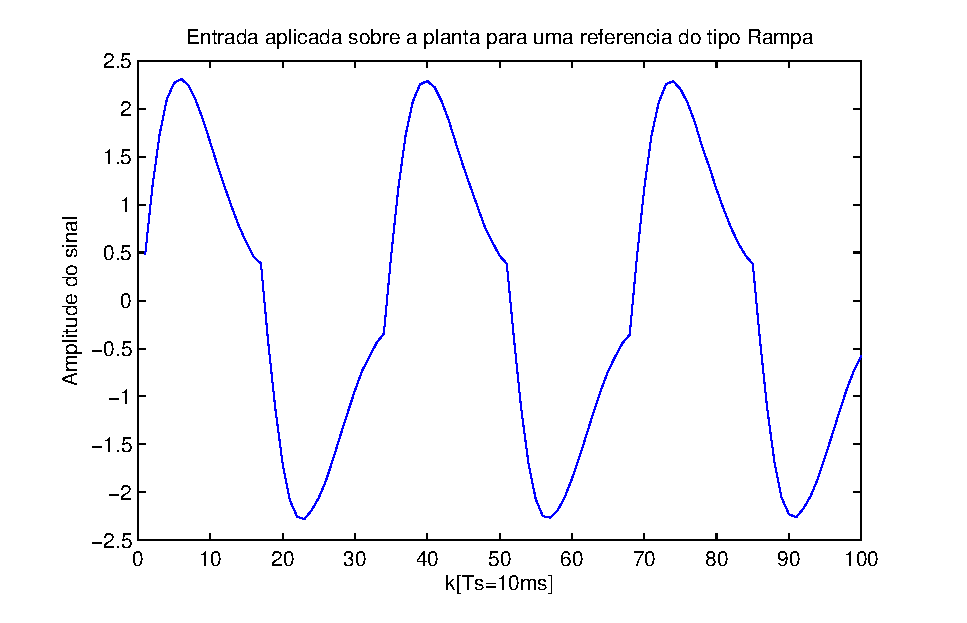
\includegraphics[width=0.98\columnwidth]{figures/input_data1_v_ramp.eps}
	\caption{Entrada aplicada sobre o sistema $G(q)$ quando submetido a uma referencia
	do tipo rampa.}
	\label{fig:in_v1_rampa}
\end{figure}

\begin{figure}[htbp]
	\center
	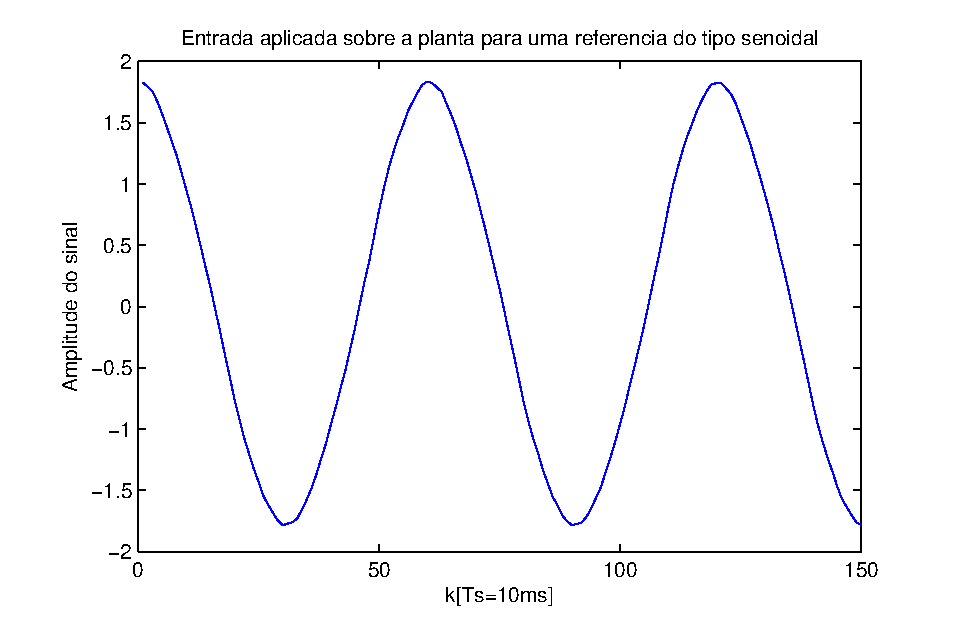
\includegraphics[width=0.98\columnwidth]{figures/input_data2_v_sin.eps}
	\caption{Entrada aplicada sobre o sistema $G(q)$ quando submetido a uma referencia
	do tipo senoidal.}
	\label{fig:in_v2_sin}
\end{figure}

\begin{figure}[htbp]
	\center
	\includegraphics[width=0.98\columnwidth]{figures/input_data3_v_ramp.eps}
	\caption{Entrada aplicada sobre o sistema $G(q)$ quando submetido a uma referencia
	do tipo rampa.}
	\label{fig:in_v3_rampa}
\end{figure}

\begin{figure}[htbp]
	\center
	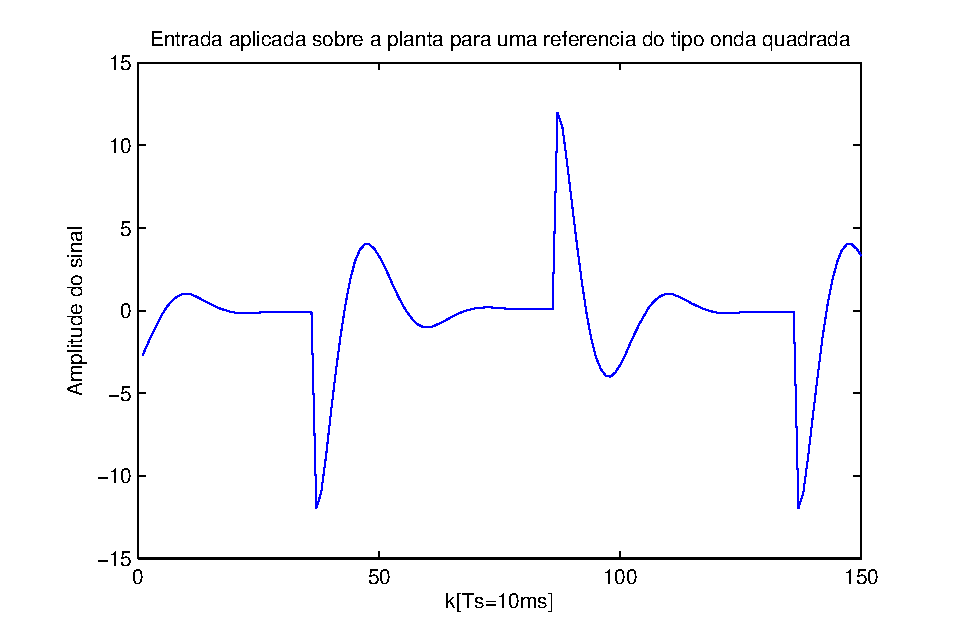
\includegraphics[width=0.98\columnwidth]{figures/input_data4_v_quad.eps}
	\caption{Entrada aplicada sobre o sistema $G(q)$ quando submetido a uma referencia
	do tipo onda quadrada.i}
	\label{fig:in_v4_quad}
\end{figure}

A figura (\ref{fig:mmq_d1_ramp}) apresenta os valores estimados para o sistema quando
submetido a uma referencia do tipo rampa, assim como na figura (\ref{fig:mmq_d3_ramp}), 
a diferenca entre ambos os sinais � a frequencia da onda de refer�ncia.

Na figura (\ref{fig:mmq_d4_quad}) � apresentado os resultados para a estimativa do sistema
quando a refer�ncia para o sistema � uma onda quadrada.

\begin{figure}[htbp]
	\center
	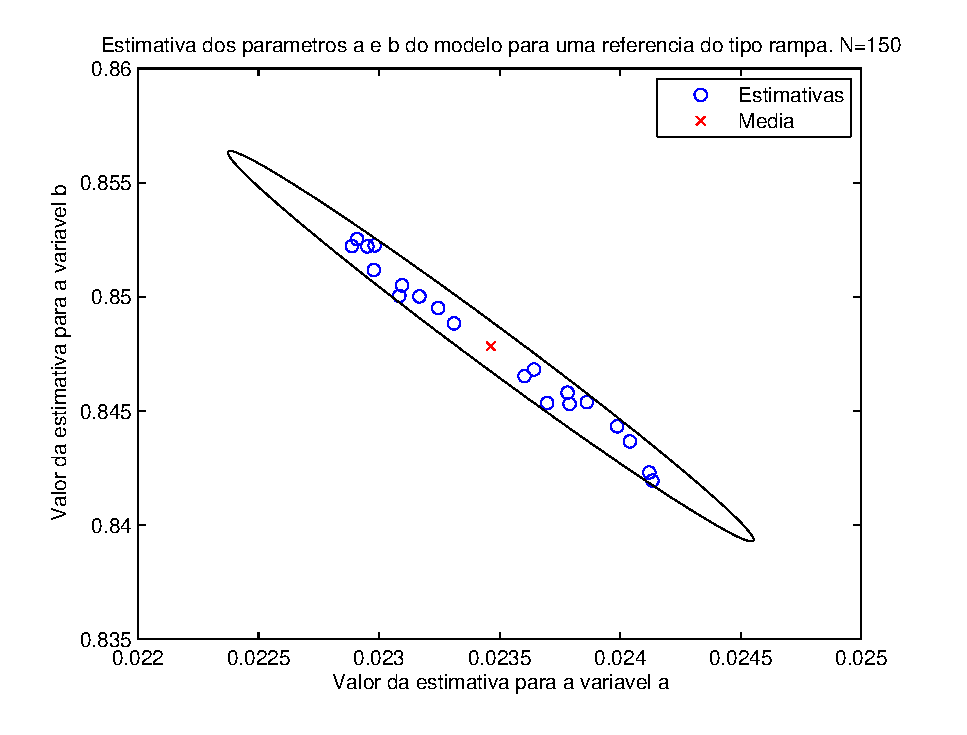
\includegraphics[width=0.98\columnwidth]{figures/mmq_d1_ramp_n150.eps}
	\caption{Estimativas das vari�veis a e b para o conjunto de dados 1.}
	\label{fig:mmq_d1_ramp}
\end{figure}


\begin{figure}[htbp]
	\center
	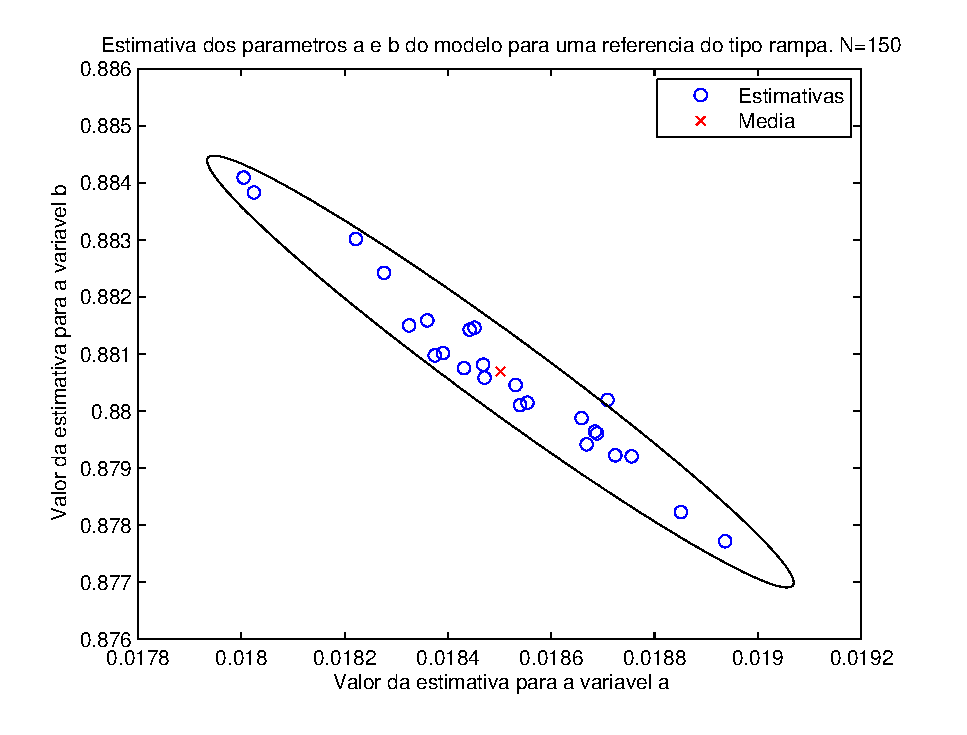
\includegraphics[width=0.98\columnwidth]{figures/mmq_d3_ramp_n150.eps}
	\caption{Estimativas das vari�veis a e b para o conjunto de dados 3.}
	\label{fig:mmq_d3_ramp}
\end{figure}

\begin{figure}[htbp]
	\center
	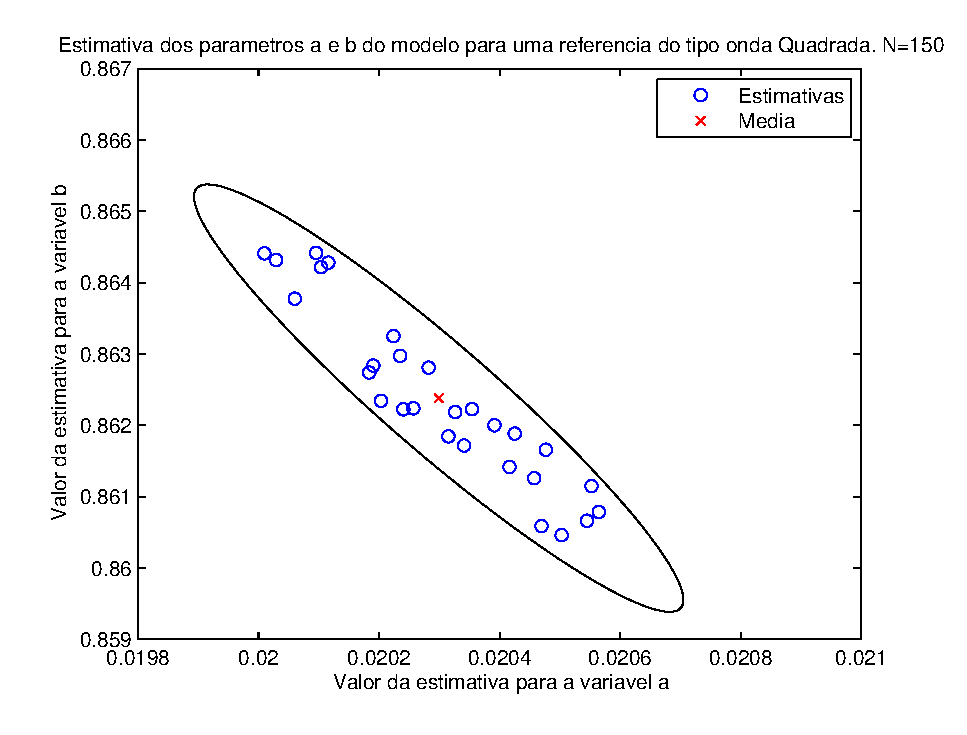
\includegraphics[width=0.98\columnwidth]{figures/mmq_d4_quad_n150.eps}
	\caption{Estimativas das vari�veis a e b para o conjunto de dados 4.}
	\label{fig:mmq_d4_quad}
\end{figure}

Para o caso quando temos na entrada do sistema uma senoide puramente, n�o � poss�vel
estimar os parametros do modelo sem que haja erro de polarizac�o. Isso � devido ao 
fato de que a entrada do sistema n�o � suficientemente excitavel para o sistema.
Obtem-se desta forma valore defasados dos que foram obtidos com as outras entradas
aplicadas sobre o sistema.

\begin{figure}[htbp]
	\center
	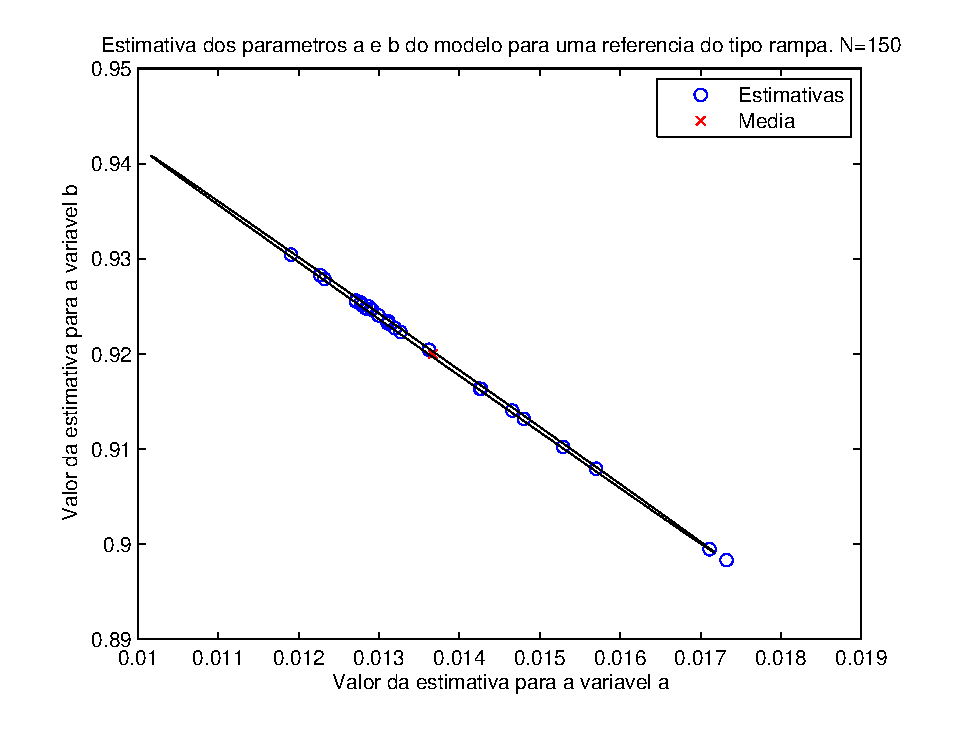
\includegraphics[width=0.98\columnwidth]{figures/mmq_d2_sin_n150.eps}
	\caption{Estimativas das vari�veis a e b para o conjunto de dados 2.}
	\label{fig:mmq_d2_sin}
\end{figure}

Na tabela (\ref{tab:mmq_results}) � apresentado os valores encontrados para cada conjunto
de dados. Apresenta-se tamb�m para quest�es de exemplificar, o resultado obtido quando
altera-se o tamanho do conjunto de dados que � utilizado para estimar os parametros.

\begin{table}[htbp]
  \begin{center}
	\caption{Valores estimados de $G(q)$ para o m�todo dos min�mos quadrados (ARX)}
	\label{tab:mmq_results}
	\begin{small}
	  \begin{tabular}{lcll}
		\hline
		Conjunto	& N      & Media a & Media b  \\
		\hline
		1 - Rampa	& 150     &  0.0235 & 0.8478   \\
		1 - Rampa	& 300     &  0.0234 & 0.848    \\
		1 - Rampa	& 600     &  0.0234 & 0.8481   \\
		1 - Rampa	& 1500    &  0.0234 & 0.8482   \\
		\hline
		2 - Sin 	& 150     &  0.0137 & 0.92     \\
		2 - Sin 	& 300     &  0.0137 & 0.92     \\
		2 - Sin 	& 600     &  0.0136 & 0.9201   \\
		2 - Sin 	& 1500    &  0.0135 & 0.9209   \\
		\hline
		3 - Rampa	& 150     & 0.0185  & 0.8807   \\
		3 - Rampa	& 300     & 0.0185  & 0.8807   \\
		3 - Rampa	& 600     & 0.0185  & 0.8807   \\
		3 - Rampa	& 1500    & 0.0185  & 0.8808   \\
		\hline
		4 - Quadrada & 150    & 0.0203  & 0.8624   \\
		4 - Quadrada & 300    & 0.0203  & 0.8624   \\
		4 - Quadrada & 600    & 0.0203  & 0.8624   \\
		4 - Quadrada & 1500   & 0.0202  & 0.8629   \\
		\hline
	  \end{tabular}
	\end{small}
  \end{center}
\end{table}



\subsubsection{Resultados para um modelo incompleto}
%===============================================================================

Nesta se��o ser� apresentado resultados para uma estimativa utilizando um modelo que n�o consegue
descrever o sistema propriamente. Ser�o utilizados os mesmos dados da estimativa do item anterior.

O modelo utilizado � descrito em (\ref{eq:mmq_motor_arx_inc}). Observa-se que o integrador n�o esta presente
neste modelo, desta forma tem-se que o modelo das vari�veis a serem utilizadas no m�todo dos 
m�nimos quadrados fica como em (\ref{eq:mmq_arx_inc_var}).

\begin{equation}
G(q, \theta)=\frac{a}{(q-b)} \;\;H(q, \theta)=\frac{q}{(q-b)}
\label{eq:mmq_motor_arx_inc}
\end{equation}

\begin{equation}
\begin{matrix}
\theta = \begin{bmatrix}
a & b 
\end{bmatrix}
&
\varphi (t)=\begin{bmatrix}
r(t-1)\\ 
y(t-1) 
\end{bmatrix}
\end{matrix}
\label{eq:mmq_arx_inc_var}
\end{equation}

Para este modelo chegou-se aos valores dos par�metros $a$ e $b$ apresentados na 
Figura (\ref{fig:mmq_arx_inc}).

\begin{figure}[htbp]
	\center
	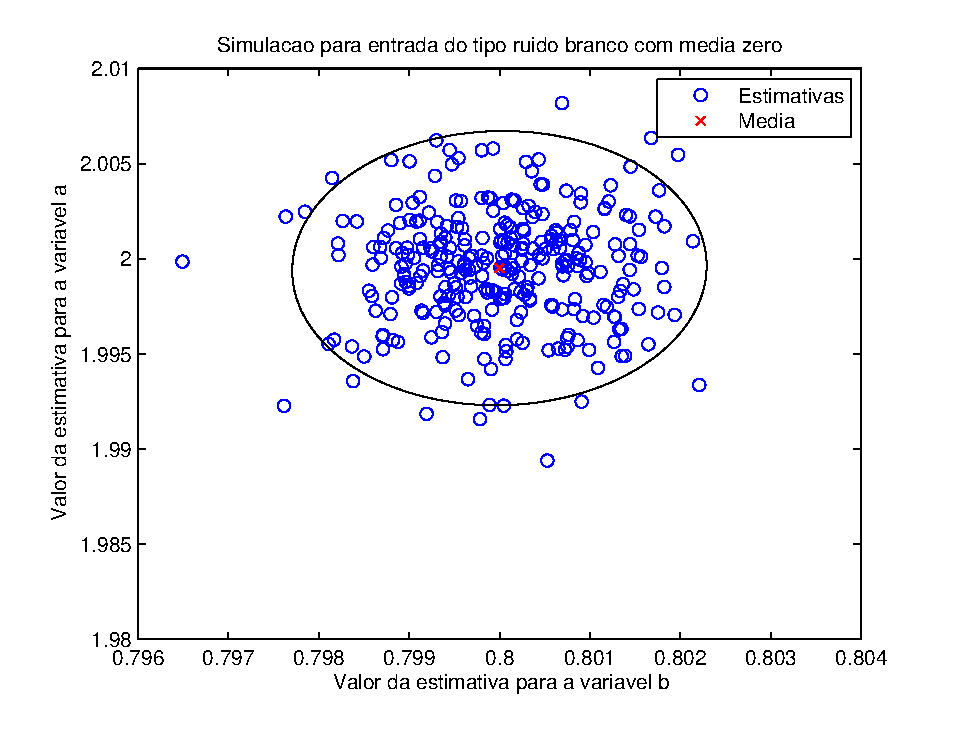
\includegraphics[width=0.98\columnwidth]{figures/mmq_arx.eps}
	\caption{TODO}
	\label{fig:mmq_arx_inc}
\end{figure}


\section{Classes de modelos Gen�ricas}
\label{sec:non_arx}
%===============================================================================



\section{Conclus�es}
\label{sec:concl}

O projeto de controladores denominados Robustos � uma �rea bem abrangente e com
in�meras aplica��es na engenharia de controle. Sistemas sujeitos a incertezas s�o
praticamente todos os sistemas f�sicos, alguns com mais e outros com menos intensidade
e representatividade da incerteza apresentada. Estas incertezas como vimos pode ser
de v�rias origens (Se��o \ref{sec:caracterization}) e s�o classificadas em tipos. Neste
trabalho apresentamos a modelagem matem�tica de 4 tipos, considerados principais e
que cobrem boa parte das incertezas mais encontradas.

Incertezas do tipo polit�picas (Se��o \ref{sec:carac_politopica}) formam uma regi�o em forma de 
um politopo, e para se encontrar uma realimenta��o de estados para este sistema � 
necess�rio que o sistema seja est�vel em todos os v�rtices deste politopo. Nas se��es 
\ref{sec:normh2_politopico} e \ref{sec:hinf_sis_politopico} foi apresentado uma
realimenta��o de estados para incertezas deste tipo tendo como requisitos as normas 
$H_2$ e $H_{\infty}$ respectivamente. Foi observado pelas Figuras (\ref{fig:h2_polytopic})
e (\ref{fig:hinf_polytopic}) que o sistema que � submetido a norma $H_2$ possui um
sobrepasso maior para uma entrada do tipo degrau, e um tempo de acomoda��o maior
se comparado com o sistema sujeito a norma $H_{\infty}$.

Incertezas do tipo limitadas em norma (Se��o \ref{sec:carac_limit_norma}) onde n�o se tem 
informa��es detalhadas sobre os componentes do sistema. Para este tipo de incerteza se 
encontrou uma realimenta��o de estados sujeito as normas $H_2$ e $H_{\infty}$ e 
nas Figuras (\ref{fig:h2_norm_bounded}) e (\ref{fig:hinf_norm_bounded}) observa-se o
comportamento do sistema nos dois casos, com o sistema no centro das incertezas e tamb�m 
em algum dos v�rtices das incertezas.

Apresentou-se tamb�m a modelagem matem�tica para incertezas do tipo Diagonais 
(Se��o \ref{sec:carac_diagonais}) e elemento a elemento (Se��o \ref{sec:carac_elemento}).

Sa Se��o \ref{sec:robust} foi apresentado resumidamente a modelagem matem�tica utilizada
para resolver o problema de estabilidade dos sistemas sujeitos a cada uma das incertezas
retratadas neste trabalho.

Para a resolu��o dos problemas de incertezas para cumprimento das normas especificadas
foi utilizado o Solver de LMI \cite{lmi_matlab} do Matlab. A ferramenta � muito interessante e facilita 
muito o projeto e resolu��o da problem�tica que envolve sistemas mais complexos e com
mais incertezas em sua formula��o.

Controladores robustos s�o muitas vezes n�o s� desejados, mas tamb�m necess�rios em certos
tipos de aplica��es. Desta forma o estudo de modelagem, caracteriza��o e resolu��o destes
problemas se torna muito importante. O conhecimento matem�tico dos m�todos que as ferramentas
atuais utilizam para resolu��o dos problemas � tamb�m muito importante e �til para 
qualquer engenheiro que venha a se deparar com problemas incertos e com requisitos de
confiabilidade elevados.



%===============================================================================
\appendix
%===============================================================================
\chapter{1 - Script para Simula��o do MQ para o modelo ARX} 
\label{appendix_mmq}
\lstset{caption=M�todo dos m�nimos quadrados,label=DescriptiveLabel}
\lstinputlisting{matlab_files/simul.m}

%===============================================================================
\chapter{2 - Script para Simula��o do m�todo das vari�veis instrumentais} 
\label{appendix_iv}
\lstset{caption=M�todo das vari�veis instrumentais,label=DescriptiveLabel}
\lstinputlisting{matlab_files/simul_iv.m}

%===============================================================================
\chapter{3 - Script para Simula��o do m�todo dos minimos quadrados considerando o PID} 
\label{appendix_mmq_pid}
\lstset{caption=M�todo dos minimos quadrados considerando-se o controlador PID,label=DescriptiveLabel}
\lstinputlisting{matlab_files/simul_pid.m}

%===============================================================================


\bibliographystyle{IEEEtran}
\bibliography{biblio}

\end{document}
